### The Connection Between the "S Matrix" and the Function `mgcv::smooth2random`

#### Introduction

In statistical modeling, particularly in Generalized Additive Models (GAMs), the "  S matrix" is a penalty matrix that is used to impose smoothness constraints on the estimated functions. The function `mgcv::smooth2random` in the R package `mgcv` is used to convert a smooth term into a random effect, facilitating its use in mixed models like those fitted by `glmmTMB`.

#### Mathematical Description

Let \( S \) be the penalty matrix for a smooth term, defined in the original scale. This matrix is used to penalize the wiggliness of the smooth term. The penalty term is given by:

\[
\text{Penalty} = \mathbf{b}^T S \mathbf{b}
\]

where \( \mathbf{b} \) is the vector of basis function coefficients.

The function `mgcv::smooth2random` transforms this smooth term into a random effect by providing a transformation matrix \( A \) and its diagonal matrix \( D \). The transformation is defined as:

\[
\mathbf{b}_{\text{fit}} = A^{-1} \mathbf{b}_{\text{original}}
\]

The penalty term in the fit scale becomes:

\[
\text{Penalty}_{\text{fit}} = \mathbf{b}_{\text{fit}}^T \mathbf{b}_{\text{fit}} = \mathbf{b}_{\text{original}}^T (A^{-1})^T A^{-1} \mathbf{b}_{\text{original}}
\]

Thus, we can relate \( S \) and \( A \) as:

\[
S = (A^{-1})^T A^{-1}
\]

#### Code Explanation

1. **Setting up the smooth term**: The code uses `mgcv::smoothCon` to set up a penalized thin-plate regression spline for a continuous covariate \( x \).

    ```R
    sm <- mgcv::smoothCon(s(x), data=as.data.frame(x))[[1]]
    ```

2. **Extracting the S matrix**: The penalty matrix \( S \) is extracted from `sm$S[[1]]`. Some rows and columns are removed for specific reasons related to the model.

    ```R
    S <- sm$S[[1]][-(9:10),-(9:10)]
    ```

3. **Transforming to Random Effect**: The `mgcv::smooth2random` function is used to get the transformation matrix \( A \) and its diagonal \( D \).

    ```R
    re <- mgcv::smooth2random(sm, "", type=2)
    A <- (re$trans.U %*% diag(re$trans.D))[-(9:10),-(9:10)]
    ```

4. **Verifying the Relationship**: The code verifies that \( S = (A^{-1})^T A^{-1} \).

    ```R
    S - t(solve(A))%*%solve(A)
    ```

#### Conclusion

The code demonstrates the mathematical relationship between the penalty matrix \( S \) in the original scale and the transformation matrix \( A \) in the fit scale. This relationship is crucial for understanding how smooth terms can be incorporated as random effects in mixed models.

You can copy and paste this explanation directly into Overleaf for your documentation or thesis work.

Ben Bolker, using the s2rPred function has so far accomplished the following. 
\newline

\subsection*{Successful Parts:}

\begin{enumerate}[label=\arabic*.]
    \item \textbf{Model Fitting:}
    \begin{itemize}
        \item Both \texttt{mgcv} and \texttt{glmmTMB} have been successfully used to fit models to the \texttt{sleepstudy} dataset.
        \item The \texttt{Nile} dataset has also been used to fit models using both packages.
    \end{itemize}
    
    \item \textbf{Data Transformation:}
    \begin{itemize}
        \item The \texttt{sleepstudy} and \texttt{Nile} datasets have been successfully loaded and transformed for analysis.
    \end{itemize}
    
    \item \textbf{Visualization:}
    \begin{itemize}
        \item A custom plotting function (\texttt{pfun}) has been created to visualize the relationship between starting \texttt{theta} values and estimated \texttt{theta} values for a series of models.
    \end{itemize}
    
    \item \textbf{Comparisons:}
    \begin{itemize}
        \item Log-likelihoods of the two models (\texttt{mgcv1} and \texttt{gtmb1}) have been compared.
        \item Fixed effects, random effects, fitted values, and predicted values of the models have been compared using the \texttt{all.equal} function.
    \end{itemize}
\end{enumerate}


\subsection{Viability of \(X_r\) Terms (speculation)}

The \(X_r\) terms offer a flexible way to model complex relationships. They combine the benefits of smooth terms and random effects, providing a nuanced understanding of the data (??).

\subsection{Splines and Basis Function Expansions}

\subsubsection{Mathematical Description}

\textbf{Splines:} A spline is a piecewise-defined polynomial function. In the simplest case, a spline \( S(x) \) of degree \( k \) is defined as:

\[
S(x) = \begin{cases} 
P_1(x) & \text{for } x \in [a_1, a_2) \\
P_2(x) & \text{for } x \in [a_2, a_3) \\
\vdots \\
P_n(x) & \text{for } x \in [a_n, a_{n+1}]
\end{cases}
\]

where \( P_i(x) \) are polynomial functions of degree \( k \) and \( a_1, a_2, \ldots, a_{n+1} \) are the knots that partition the domain.

\textbf{Basis Function Expansions:} A basis function expansion represents a function \( f(x) \) as a linear combination of basis functions \( \phi_i(x) \):

\[
f(x) = \sum_{i=1}^{n} \beta_i \phi_i(x)
\]

The basis functions \( \phi_i(x) \) can be any set of functions, not necessarily polynomials.

\subsubsection{Intuitive Description (chatGPT)}

\textbf{Splines:} Imagine you have several small sticks (polynomials) and you want to lay them end-to-end to approximate a curve. Each stick can bend or curve within its own region, but it must meet the next stick smoothly at the "knots." This is essentially what a spline does. It uses piecewise polynomials to approximate complex curves.

\textbf{Basis Function Expansions:} Think of basis function expansions like building blocks. You have a set of basic shapes (basis functions), and you can scale and add them together to approximate any shape (function) you like. These basis functions could be anything—polynomials, sine and cosine functions, etc.

\subsubsection{Differences}

\textbf{Mathematically:}
\begin{itemize}
    \item Splines are constrained to be piecewise polynomials, whereas basis function expansions can use any set of functions as basis.
    \item Splines require the polynomials to be smooth at the knots, but basis function expansions have no such requirement.
\end{itemize}

\textbf{Intuitively:}
\begin{itemize}
    \item Splines are like a smooth road made of small, connected segments, each with its own curvature.
    \item Basis function expansions are like a mosaic made up of various shapes that together form a complete picture.
\end{itemize}

\subsubsection{Conclusion}

While splines are a specific type of basis function expansion using piecewise polynomials, basis function expansions are more general and can use any set of functions as basis. Both are powerful tools for approximating complex functions, but they differ in flexibility and constraints.
\subsection{Comparing gtmb0 and gamm\_model in R}

\subsubsection{Summaries and AIC/BIC}

The summary prints for the models suggest that they are quite similar, but due to the structure, complexity and size of the models, it's not an obvious conclusion that the models are equivalent, since the format of the summary prints are quite different and include very many terms. 
\newline
Also no AIC or BIC was possible to compute for the \texttt{gamm\_model}, so we have nothing to compare the scores of \texttt{gtmb0} to. 

\subsubsection{Residual plots}

insert plots here

\subsubsection{Calculating RMSE for the models}

We have used the \texttt{"caTools"} package to split our data into a training set and a testing set, and then refit our models to be able to calculate their root mean squared error (RMSE). Code in Appendix. 
\newline

 RMSE is defined as:

\[
\text{RMSE} = \sqrt{\frac{1}{n} \sum_{i=1}^{n} (y_i - \hat{y}_i)^2}
\]

Where \(y_i\) is the actual value, \(\hat{y}_i\) is the predicted value, and \(n\) is the number of observations.
\newline

We get the following RMSE prints 

\begin{verbatim}
    "RMSE for gtmb0:       11.157443"
    "RMSE for gamm_model:  11.199512"
\end{verbatim}

These values are very close. 

\subsubsection{Equivalence testing}

Using the \texttt{"TOSTER"} package to perform Two One-Sided Tests (TOST) using the \texttt{tusm\_TOST()} function (code in Appendix). 
\newline

\begin{enumerate}
    \item \textbf{Equivalence Test}: The equivalence test was significant with \( t(1144) = 3.385 \) and \( p = 3.68 \times 10^{-4} \). This implies that the null hypothesis of non-equivalence can be rejected, suggesting that the residuals from the two models (`gtmb0` and `gamm\_model`) are statistically equivalent within the predefined bounds.
    
    \item \textbf{Null Hypothesis Significance Test (NHST)}: The null hypothesis test was non-significant with \( t(1144) = -6.837 \times 10^{-13} \) and \( p = 1 \). This implies that the null hypothesis that the effect is equal to zero is not rejected, indicating that there is no significant difference between the residuals of the two models.
    
    \item \textbf{Effect Sizes}: The raw estimate and Hedges's \( g \) are both extremely close to zero, further supporting the idea that the two models are equivalent in terms of their residuals.
\end{enumerate}

\subsubsection{Interpretation}

\begin{itemize}
    \item \textbf{NHST}: The non-significant result in the null hypothesis significance test suggests that there is no significant difference between the residuals of the two models. This is what would be expected if the models are indeed similar.
    
    \item \textbf{TOST}: The significant result in the equivalence test indicates that not only are the residuals from the two models not significantly different, but they are also statistically equivalent within the predefined bounds. This is strong evidence that the two models are producing very similar results.
    
    \item \textbf{Effect Sizes}: The effect sizes are negligible, which is consistent with the other tests and supports the conclusion of equivalence.
\end{itemize}

\subsubsection{Testing a different model}
Despite the very strong evidence obtained from the 'chigaco' data models that the two models are equivalent, let's make sure by trying a different data set as well. 

The data set on trial this time is the \texttt{ipo} data from the \texttt{gamair} package. 

We think that the \texttt{ir} (initial return) variable could be of interest to predict, and that the \texttt{dp} (percentage difference) may be a strong predictor of this response, and quite possibly in a non-linear way. Hence we fit the model

\[
\text{initial retur } \sim s(percentage difference)
\]

Which translates to the following two models
   
    \[
    \text{ir} = \beta_0 + s(dp) + \epsilon
    \]
    
    
    \[
    \text{ir} = \alpha_0 + \alpha_1 Xr_{dp} + \epsilon
    \]

\textbf{Summary of TOST}

\begin{itemize}
    \item \textbf{NHST}: The p-value is 1, indicating that we fail to reject the null hypothesis that the effect is equal to zero. This suggests that the two models (\textit{gam1} and \textit{glmmTMB1}) do not significantly differ in their ability to predict \textit{ir}.
    
    \item \textbf{Equivalence Test (TOST)}: The p-value is 0.058, slightly above the alpha level of 0.05. This means that we fail to reject the null hypothesis of the equivalence test, suggesting that the data do not provide sufficient evidence to claim that the two models are equivalent within a predefined margin.
    
    \item \textbf{Effect Sizes}: Both the raw estimate and Hedges's g are essentially zero, indicating no practical difference between the two models.
\end{itemize}

The results once again suggest that the models are equivalent. 


\subsection{Comparing s() terms in glmmTMB and mgcv}
The s() terms in glmmTMB seem to have the same base we encounter in mgcv, however there are some restrictions in the functions within s().

Along with the default thin plate regression, there are several basis functions we have not encountered problems with.


\begin{table}[h]
    \centering
    \caption{TMB-appropriate \( s() \) functions}
    \label{tab:TMB-functions}
    \begin{tabularx}{\textwidth}{|c|X|}
        \hline
        Function & Description \\
        \hline 
        \( \text{bs} = \text{"cr"} \) & Cubic Regression Splines \\
        \hline 
        \( \text{bs} = \text{"ps"} \) & P-Splines, B-splines with a difference penalty to make them smooth  \\
        \hline
        \( t2(x1,x2) \) & Tensor product smooths \\
        \hline
    \end{tabularx}
\end{table}

A limited function we encounter is the knot function. In mgcv the k parameter can be set all the way down to 3, which is the same in glmmTMB, but we encounter problems when we are trying to visualize the model in summary, with the random conditional model encountering an index error.






\newline
Over to the functions we have not made progress with. Most of these we will try to explain later when we delve into Johnsons way to interpret s() functions in glmmTMB. Here are a few examples:

\begin{table}[h]
    \centering
    \caption{Not Fit for \( s() \) in TMB}
    \label{tab:NotFitForTMB}
    \begin{tabularx}{\textwidth}{|c|X|}
        \hline
        Function & Description \\
        \hline
        \( \text{bs} = \text{"re"} \) & Random Effects, used for grouping factors \\
        \hline
        \( \text{te}(x1, x2) \) &   Tensor Product Smooths. \\
        \hline
        \( \text{bs} = \text{"cs"} \) &  Simple Cubic Splines  \\
        \hline
        \( \text{bs} = \text{"cc"} \) &  Cyclical Cubic Regression Splines \\
        \hline
    \end{tabularx}
\end{table}

The reason for the problems we encounter in the different basis functions is because of the Xf-term we later will talk about in the Johnson vs Bolker section.


\subsubsection{Difference between \texttt{te()} and \texttt{t2()} in R's mgcv package}

Both \texttt{te()} and \texttt{t2()} are used for specifying tensor product smooths in generalized additive models (GAMs) using the \texttt{mgcv} package in R. However, they differ in the way they handle constraints and penalties on the basis functions.

\begin{itemize}
    \item \textbf{te()}: This function imposes identifiability constraints on the tensor product smooth. It ensures that the estimated smooth does not include components that can be represented as the sum of lower-dimensional smooths of the individual variables. This makes the model easier to interpret and is the standard choice for most tensor product smooths.
    
    \item \textbf{t2()}: This function allows for unconstrained tensor product smooths. It does not impose the identifiability constraints that \texttt{te()} does. This offers more flexibility but generally makes the model harder to interpret.
\end{itemize}

In summary, use \texttt{te()} for situations where interpretability is essential, and \texttt{t2()} when you need more flexibility and are less concerned about straightforward interpretation. The reason we can only use the \textbf{t2()} function is because te() smooths is not useable with gamm4-package.




\subsection{Comparing Xr terms and s() terms in R}

We will also compare the Xr terms we have made to a type of s() terms which have been coded directly to the \texttt{glmmTMB} package by Ben Bolker. This has however caused some issues when running the models, such as convergence failure, so we test if our method could give better results, starting with the chicago data set we have used earlier.
\newline
\begin{verbatim}
    gtmb0s <- glmmTMB(formula = death ~ s(tmpd), 
                 data = chicago, REML = TRUE)

    gtmb0Xr <- glmmTMB(formula = death ~ Xr_tmpd, 
                 data = chicago, REML = TRUE)


    gam0<- gam(formula = death ~ s(tmpd), 
           data = chicago, REML=TRUE)

        
\end{verbatim}

Comparing the summaries of the models, they are all quite similar with the covariate of temperature being decently significant. Something that is worth noticing is the difference in 1 degrees of freedom. The AIC is slightly better for the Xr terms but they are pretty similar, which we also can see from their model fits.
\newline
While analyzing the dharma residuals in the two models, we can see that the Xr terms have better residuals, but is this because they are really better, or does the s() function not work as good with the DHARMa-plots? 
From the plot of residuals versus fitted values we see that the plots are quite similar, however gtmb0Xr uses a wider range in their fitted values.

\begin{verbatim}
    "RMSE for gtmb0s:  13.0230351135241"
    "RMSE for gtmb0Xr:  13.0361758742346"
\end{verbatim}

\begin{table}[h]
\centering
\caption{Comparison of Chicago models}
\label{table:further_model_comparison}
\begin{tabular}{|c|c|c|c|}
\hline
Model & AIC & BIC & LogLik \\
\hline
gtmb0s & 41479.36 & 41505.52 & -20735.68 \\
\hline
gtmb0Xr & 41414.78 & 41480.18 & -20697.39 \\
\hline
gam0 & 41456.82 & 41522.19 & -20718.41 \\
\hline
\end{tabular}
\end{table}


\subsection{Comparing Ben Bolker and Devin Johnson method }

To implement splines in glmmTMB there have been to different approaches before. Bolker has implemented the spline function into the glmmTMB-package using some of Devin Johnsons method along with algorithms found in mgcv.

Although using REML in these two models will give similar outputs, they are not identical,  we would like to delve into how and why this occurs. We proceed using the chicago dataset to make model using Johnsons method and comparing it to gtmb0s from the section above:


\begin{verbatim}
    ftmb1 <- glmmTMB(formula = death ~ 0 + Xf_tmpd + 
    homdiag(0 + Xr_tmpd | fake_group), data = chicago,
    REML = TRUE)
        
\end{verbatim}


From the summary outputs we can see that the random conditional model is identical for these two glmmTMB-models, the spline function estimate in Bolkers method is also identical with the estimate Xftmpd1, however the intercept and Xftmpd2 are not the same, this is something we need to understand.




\subsection{Model convergence issues using s()}

When using the chicago dataset, if we want to make a model based on the p10median-variable we have to omit the variables NA-values. When we do this our basic model only using temperature as a spline will have model convergence problems, non-positive-definite Hessian matrix. Another change we see from removing the NA-values is that the second Xf-term will shift from 1 to -1, could these two differences have something to do with each other?





\subsection{Multiple \( s() \) Terms in \texttt{glmmTMB} and \texttt{mgcv}}

The terms in the model are additive, meaning they contribute independently to the response variable. The smooth terms in \texttt{glmmTMB} behave similarly to those in \texttt{mgcv}, with each \( s() \) term being additive and capturing different aspects of the relationship between the predictors and the response variable.


In \texttt{glmmTMB}, it is common to represent smooth terms as random effects with a specific covariance structure that induces smoothing. This approach allows the fitting of additive models within the mixed modeling framework. However, the assumption of additivity still holds; each term contributes independently to the model.


Similar to \texttt{mgcv}, if multiple \( s() \) terms model similar relationships or are based on similar predictors, collinearity might be an issue. When using smooth terms as random effects, it is essential to ensure that their covariance structures are identifiable.


The computational cost can be high, especially when combining complex random effects structures with multiple smooth terms. \texttt{glmmTMB} generally offers more flexibility in the kinds of random-effects structures that can be fit compared to \texttt{mgcv}, but this comes at the cost of increased computational time.


Each smooth term can be interpreted in a way similar to how one would interpret them in a GAM but now within the mixed modeling framework. Each term provides insights into how a particular predictor influences the response while accounting for the other terms in the model.


In conclusion, the multiple \( s() \) terms in \texttt{glmmTMB} work additively and independently, similar to how they work in \texttt{mgcv}. The primary difference lies in the framework—\texttt{glmmTMB} fits these models within a mixed-model framework, allowing for greater flexibility in specifying random effects. However, the same considerations regarding identifiability, interpretability, and computational complexity apply.













\subsubsection{Penalized B-Splines (P-Splines) in \texttt{mgcv}}

Penalized B-splines, commonly known as P-splines, are a versatile tool for smoothing and are often used for their computational efficiency and simplicity. In \texttt{mgcv}, P-splines are specified using the basis type \texttt{bs="ps"}.

Mathematically, a P-spline can be represented as:

\begin{equation}
    f(x) = \sum_{i=1}^{k} \beta_i B_i(x),
    \label{eq:ps_splines}
\end{equation}

where \(B_i(x)\) are the B-spline basis functions, and \(\beta_i\) are the coefficients to be estimated. The B-splines are piecewise polynomial functions defined over a sequence of knots. The degree of the polynomial is commonly 3, leading to cubic B-splines, although other degrees can be used.
\newline

What sets P-splines apart is the penalty term used for smoothing. P-splines commonly use a difference penalty on the coefficients \(\beta\), which can either be a first or second-order finite difference. For first-order differences, the penalty term is:

\begin{equation}
    \text{Penalty} = \lambda \sum_{i=2}^{k} (\beta_i - \beta_{i-1})^2
    \label{1st_order_penalty,}
\end{equation}

and for second-order differences, the penalty term is

\[
\text{Penalty} = \lambda \sum_{i=3}^{k} (\beta_i - 2\beta_{i-1} + \beta_{i-2})^2,
\]

where \(\lambda\) is the smoothing parameter that controls the strength of the penalty. Higher values of \(\lambda\) result in a smoother curve, while lower values allow for more wiggly fits.




P-splines combine the flexibility of B-splines with the simplicity of a difference penalty. They are computationally efficient, easy to implement, and can be very effective for a wide range of smoothing tasks. They are particularly useful when a balance of flexibility and smoothness in the estimated function \(f(x)\) is desired.




\subsubsection{Thin Plate Splines and Their Decomposition}

\begin{enumerate}
    \item \textbf{Full Thin Plate Spline (\texttt{bs="tp"})}:
    \begin{itemize}
        \item In a full thin plate spline, the basis functions are defined in such a way that they apply across the entire range of the data. They are more global in nature.
        \item When using the \texttt{smoothCon} \citep[pp.~327]{wood2017} and \texttt{smooth2random} \cite{mgcvmanual} functions to prepare these splines for \texttt{glmmTMB}, the decomposition usually yields only an \texttt{Xr} term, with no corresponding \texttt{Xf}.
 This is because the penalty for thin plate splines makes it difficult to naturally separate them into fixed and random components.
        \item In the context of GLMMs, the entire spline term will behave as a random effect in the model.
    \end{itemize}
    
    \item \textbf{Thin Plate Regression Splines (\texttt{bs="tp"})}:
    \begin{itemize}
        \item Similar to full thin plate splines, but they are a lower-rank approximation and hence computationally more efficient.
        \item The decomposition into \(Xf\) and \(Xr\) would depend on the specific properties of the basis functions and the penalty term. It's likely that you will also only get an \(Xr\) term.
    \end{itemize}
\end{enumerate}


\subsubsection*{Mathematical Representation of Thin Plate Regression Splines}

Thin plate regression splines are a computationally efficient approximation of full thin plate splines. They are generally represented using a subset of the basis functions used in full thin plate splines, effectively creating a lower-rank approximation. The mathematical representation can be written as:

\[
f(x) = \beta_0 + \sum_{i=1}^{m} \beta_i x_i + \sum_{j=1}^{k} \gamma_j \phi(|| x - x_{j} ||)
\]

Here, \( \beta_0 \) is the intercept, \( \beta_i \) are the coefficients for the linear terms \( x_i \), \( \gamma_j \) are the coefficients for the radial basis functions \( \phi(|| x - x_{j} ||) \), \( x_j \) are the selected knot locations, and \( k \) is the reduced rank of the spline. The radial basis function \( \phi(r) \) depends on the dimensionality and is usually more complex in higher dimensions.

This lower-rank approximation makes thin plate regression splines computationally more efficient while still retaining many desirable properties of full thin plate splines.


\subsubsection*{Mathematical Representation of Full Thin Plate Splines}

Full thin plate splines are a type of global smoother that use radial basis functions to represent the smooth. In the one-dimensional case, the mathematical representation of a full thin plate spline can be written as:

\[
f(x) = \sum_{i=1}^{n} \alpha_i \phi(|| x - x_i ||)
\]

Here, \( \phi(r) \) is a radial basis function, \( \alpha_i \) are the coefficients to be estimated, \( x_i \) are the knot locations, and \( n \) is the number of knots. The radial basis function \( \phi(r) \) is usually defined as \( r^2 \log(r) \) for \( r > 0 \) and zero otherwise. This function has desirable mathematical properties, such as rotational invariance, which makes it useful for multidimensional smoothing as well.

The complexity and global nature of these basis functions make full thin plate splines computationally intensive, especially when the number of knots is large or the dimensionality is high.



Thin plate splines are more likely to be represented entirely as random effects (\(Xr\)) in the mixed model framework when prepared for \texttt{glmmTMB} using \texttt{mgcv}'s \texttt{smoothCon} and \texttt{smooth2random}. The global nature of these splines and their penalty structure make it difficult to decompose them into separate fixed (\(Xf\)) and random (\(Xr\)) components. Thin plate regression splines however will have both components added to their model, as we see the fixed terms as the beta-values in its mathematical representation.


\subsubsection{Cyclical Cubic Splines and Comparison with Regular Cubic Splines}


The cyclical cubic spline is a special case of cubic splines where the function is constrained to be cyclic at the endpoints. This means that the function value and its first and second derivatives at the endpoints are the same, ensuring smooth transitions.



Mathematically, a cyclical cubic spline \( f(x) \) can be represented as a linear combination of cubic basis functions \( B_i(x) \) and coefficients \( \beta_i \), similar to regular cubic splines:

\[
f(x) = \sum_{i=1}^{k} \beta_i B_i(x)
\]

Here, \( k \) is the number of knots, and \( B_i(x) \) are the cubic basis functions. However, the basis functions are constructed to ensure that the function is cyclic. Specifically, they are designed so that:

\[
f(x_1) = f(x_n), \quad f'(x_1) = f'(x_n), \quad f''(x_1) = f''(x_n)
\]



The penalty term for cyclical cubic splines is usually based on the integrated squared second derivative, similar to regular cubic splines:

\[
\text{Penalty} = \lambda \int [f''(x)]^2 \, dx
\]

However, the penalty matrix would be constructed to reflect the cyclical nature of the spline, taking into account the constraints at the endpoints.


\paragraph{Cubic Smoothing Splines (\texttt{bs="cs"})}

Cubic smoothing splines are designed to model data without any specific constraints at the endpoints. These splines are often smoother due to a different penalty term that targets the entire curve. When decomposed for use in \texttt{glmmTMB} through \texttt{mgcv}'s \texttt{smoothCon} and \texttt{smooth2random} functions, cubic smoothing splines do not decompose into a fixed (\(X_f\)) component. This is because the penalty term for smoothing splines makes it difficult to naturally separate them into fixed and random components.

\paragraph{Cubic Cyclical Splines (\texttt{bs="cc"})}

Cubic cyclical splines are constrained to have the same function value at both endpoints. They are useful for modeling cyclical or seasonal data. This cyclical constraint often leads to a single \(X_f\) term that captures the constant cyclical effect across the data range. The \(X_f\) term essentially represents a fixed effect to ensure the function is smooth and equal at both ends.










Penalized regression is a class of techniques in statistical modeling that introduces a penalty term to the objective function, usually the residual sum of squares (RSS), to control the complexity of the model. The general form of a penalized regression model can be written as:

\begin{equation}
\text{Minimize} \quad \sum_{i=1}^{n} (y_i - \mathbf{x}_i^T \boldsymbol{\beta})^2 + \lambda J(\boldsymbol{\beta})
\end{equation}
 \cite{wood2017}
 \newline
Here, \( \lambda \) is the smoothing parameter, and \( J(\boldsymbol{\beta}) \) is the penalty term. The penalty term serves to regularize or shrink the estimated coefficients \( \boldsymbol{\beta} \) towards zero or each other, thereby reducing the model's complexity and potential for overfitting.
Penalized regression also helps with stability in cases where there are more predictors than observations, and also makes the model more interpretable.





\subsubsection*{Comparison of the Two Penalties}

\textbf{Similarities:}
\begin{itemize}
    \item Both penalties involve a regularization parameter \( \lambda \) that controls the extent of the penalty applied.
    \item Both aim to prevent overfitting by imposing constraints on the function, though in different ways.
    \item They are both commonly used in the context of regression smoothing and can be incorporated into various types of models, including linear models and splines.
\end{itemize}

\textbf{Differences:}
\begin{itemize}
    \item The Ridge penalty focuses on the magnitude of the function, penalizing large values of the function itself. It is more about keeping the function values close to zero.
    \item The Integrated Squared Second Derivative penalty targets the curvature or the wiggliness of the function, penalizing the variability in the function's slope. It is concerned with how rapidly the function changes.
    \item As a result, the Ridge penalty tends to produce functions that are small in magnitude, while the ISSD penalty results in functions that are smoother with less rapid changes in slope.
\end{itemize}

\subsubsection{The smoothing parameter}

The smoothing parameter, often denoted by \( \lambda \), plays a crucial role in controlling the trade-off between fitting the data well and keeping the model smooth or simple. The smoothing parameter is a non-negative scalar that multiplies the penalty term in the objective function of penalized regression models. Choosing an optimal \( \lambda \) is often done via cross-validation;


\begin{itemize}
    \item \( \lambda = 0 \): No penalty is applied, and the model reduces to ordinary least squares regression for linear models or a non-penalized generalized additive model for GAMs. This could lead to overfitting if the model is complex.
    \item \( \lambda \) is large: A strong penalty is applied, which can lead to underfitting. In the extreme, all coefficients may be pushed towards zero, resulting in a model that is too simple to capture the underlying pattern in the data.
    \item \( \lambda \) is moderate: A balance is struck between fitting the data and keeping the model smooth or simple. This is often the desired scenario and is usually determined through techniques like cross-validation.
\end{itemize}

In the context of smoothing splines, \( \lambda \) controls the smoothness of the fitted curve. A large \( \lambda \) will result in a smoother curve, while a small \( \lambda \) will allow for more wiggles, capturing more of the data's fine-grained structure.

In GAMs, \( \lambda \) can be different for each smooth term, allowing for varying levels of smoothness for different predictors. This is particularly useful when dealing with high-dimensional data or when different predictors have different scales or units.




The general form of a \textbf{glmm} can be expressed as:

\[
g(\mu_{ij}) = \mathbf{X}_{ij} \boldsymbol{\beta} + \mathbf{Z}_{ij} \mathbf{u}_{j}
\]

Where:
- \( g() \) is the link function that relates the mean \( \mu \) of the response variable to the linear predictors.
- \( \mathbf{X}_{ij} \) is the design matrix for fixed effects.
- \( \boldsymbol{\beta} \) is the vector of fixed effect parameters.
- \( \mathbf{Z}_{ij} \) is the design matrix for random effects.
- \( \mathbf{u}_{j} \) is the vector of random effect parameters for the \( j^{th} \) group.

The random effects \( \mathbf{u}_{j} \) are typically assumed to be normally distributed with mean zero and some covariance matrix \( \mathbf{G} \) (the covariance matrix will later be denoted by $\Sigma$, and also become highly relevant):

\[
\mathbf{u}_{j} \sim \mathcal{N}(0, \mathbf{G})
\]

Zero-inflated models account for excess zeros in the data. A zero-inflated Poisson (ZIP) model, for example, can be expressed as:

\[
y_{ij} = 
\begin{cases} 
0 & \text{with probability } \psi + (1-\psi)e^{-\lambda_{ij}} \\
k & \text{with probability } (1-\psi)\frac{\lambda_{ij}^k e^{-\lambda_{ij}}}{k!} \text{ for } k=1,2,\ldots
\end{cases}
\]

Where \( \lambda_{ij} \) is the Poisson rate for observation \( i \) in group \( j \), and \( \psi \) is the zero-inflation parameter.



In LMMs, REML offers a powerful approach for analyzing hierarchical and clustered data. By accounting for both fixed and random effects, LMMs effectively model complex data, while REML ensures unbiased variance component estimation. These methods are widely applicable across various fields, including biology, economics, and social sciences.






\subsection{The Connection Between the "S Matrix" and the Function \texttt{mgcv::smooth2random}}

\subsubsection{Introduction}

In statistical modeling, particularly in Generalized Additive Models (GAMs), the "S matrix" is a penalty matrix that is used to impose smoothness constraints on the estimated functions. The function \texttt{mgcv::smooth2random} in the R package \texttt{mgcv} is used to convert a smooth term into a random effect, facilitating its use in mixed models like those fitted by \texttt{glmmTMB}.

\subsubsection{Mathematical Description}

Let \( S \) be the penalty matrix for a smooth term, defined in the original scale. This matrix is used to penalize the wiggliness of the smooth term. The penalty term is given by:

\[
\text{Penalty} = \mathbf{b}^T S \mathbf{b}
\]

where \( \mathbf{b} \) is the vector of basis function coefficients.

The function \texttt{mgcv::smooth2random} transforms this smooth term into a random effect by providing a transformation matrix \( A \) and its diagonal matrix \( D \). The transformation is defined as:

\[
\mathbf{b}_{\text{fit}} = A^{-1} \mathbf{b}_{\text{original}}
\]

The penalty term in the fit scale becomes:

\[
\text{Penalty}_{\text{fit}} = \mathbf{b}_{\text{fit}}^T \mathbf{b}_{\text{fit}} = \mathbf{b}_{\text{original}}^T (A^{-1})^T A^{-1} \mathbf{b}_{\text{original}}
\]

Thus, we can relate \( S \) and \( A \) as:

\[
S = (A^{-1})^T A^{-1}
\]

\subsubsection{Code Explanation}

\begin{enumerate}
    \item \textbf{Setting up the smooth term}: The code uses \texttt{mgcv::smoothCon} to set up a penalized thin-plate regression spline for a continuous covariate \( x \).
    \begin{verbatim}
    sm <- mgcv::smoothCon(s(x), data=as.data.frame(x))[[1]]
    \end{verbatim}

    \item \textbf{Extracting the S matrix}: The penalty matrix \( S \) is extracted from \texttt{sm\$S[[1]]}. Some rows and columns are removed for specific reasons related to the model.
    \begin{verbatim}
    S <- sm$S[[1]][-(9:10),-(9:10)]
    \end{verbatim}

    \item \textbf{Transforming to Random Effect}: The \texttt{mgcv::smooth2random} function is used to get the transformation matrix \( A \) and its diagonal \( D \).
    \begin{verbatim}
    re <- mgcv::smooth2random(sm, "", type=2)
    A <- (re$trans.U %*% diag(re$trans.D))[-(9:10),-(9:10)]
    \end{verbatim}

    \item \textbf{Verifying the Relationship}: The code verifies that \( S = (A^{-1})^T A^{-1} \).
    \begin{verbatim}
    S - t(solve(A))%*%solve(A)
    \end{verbatim}
\end{enumerate}

\subsubsection{Conclusion}

The code demonstrates the mathematical relationship between the penalty matrix \( S \) in the original scale and the transformation matrix \( A \) in the fit scale. This relationship is crucial for understanding how smooth terms can be incorporated as random effects in mixed models.





In this method, we extract the random effect representation \(X_r\) of the smooth term and use it as a fixed effect in our model. Essentially, we are fitting the model:

\begin{equation}
y = X_r \beta + \epsilon
\end{equation}

Here, \(X_r\) is the design matrix for the smooth term, \(\beta\) is the vector of coefficients, and \(\epsilon\) is the error term.

\subsection{Ben Bolker's Method: \(y \sim (X_r | \text{dummy})\)}

Ben Bolker's approach integrates smooth terms directly into the \texttt{glmmTMB} package. The smooth term is represented in both the fixed and random effects part of the model. The model can be represented as:

\begin{equation}
y = X_f \beta_f + Z \beta_r + \epsilon
\end{equation}

Here, \(y\) is the \(n \times 1\) response vector, \(X_f\) is the \(n \times q\) design matrix for the fixed effects, \(Z\) is the \(n \times m\) design matrix for the random effects (which includes the smooth terms), \(\beta_f\) is the \(q \times 1\) vector of fixed effect coefficients, \(\beta_r\) is the \(m \times 1\) vector of random effect coefficients, and \(\epsilon\) is the \(n \times 1\) error term.

The likelihood function is augmented with a penalty term \(P\):

\begin{equation}
L(y | \beta_f, \beta_r) \propto e^{-\frac{1}{2} \beta_r^T S \beta_r}
\end{equation}

Where \(S\) is the penalty matrix, which is used to smooth the curve.

We have a penalty matrix \(S\) and a basis function matrix \(B\). The smooth term can be represented as:

\begin{equation}
s(x) = B \alpha
\end{equation}

Where \( \alpha \) is the vector of smooth coefficients. The penalty term for the smooth is:

\begin{equation}
P = \alpha^T S \alpha
\end{equation}


e.g cubic splines, the penalty matrix \( S \) is typically a diagonal matrix with the first few diagonal elements set to zero. These zero elements correspond to the basis functions that make up the polynomial part of the spline (usually the intercept and the linear term). The remaining diagonal elements are positive and impose a penalty on the curvature of the spline.


\begin{equation}
S = \begin{pmatrix}
0 & 0 & 0 & 0 \\
0 & 0 & 0 & 0 \\
0 & 0 & \lambda_1 & 0 \\
0 & 0 & 0 & \lambda_2
\end{pmatrix}
\end{equation}

Here, \( \lambda_1 \) and \( \lambda_2 \) are positive penalty terms.

In Bolker's method, the first two rows and columns from \( S \) are moved to the fixed effect model matrix \( X_f \). Because these rows and columns are zeros, moving them doesn't change the penalty imposed by \( S \). Instead, it changes how these terms are estimated:

- In the \( y \sim X_r \) method, these terms are estimated as fixed effects without any penalty.
- In the \( y \sim (X_r | \text{dummy}) \) method, these terms are estimated as fixed effects but are also subject to the penalty imposed by the random effects structure.
\newline

 Let's assume \(S_1\) represents these first two rows and columns, and \(S_2\) represents the remaining part of \(S\).

\begin{equation}
S = \begin{pmatrix}
S_1 & 0 \\
0 & S_2
\end{pmatrix}
\end{equation}

The corresponding basis function matrix \(B\) can also be partitioned as \(B = [B_1, B_2]\), where \(B_1\) corresponds to \(S_1\) and \(B_2\) corresponds to \(S_2\).

The smooth term \(s(x)\) can then be partitioned as:

\begin{equation}
s(x) = B_1 \alpha_1 + B_2 \alpha_2
\end{equation}

Here, \(\alpha_1\) would be treated as fixed effects and \(\alpha_2\) as random effects.


The GLMM is updated to:

\begin{equation}
y = X_f \beta_f + B_1 \alpha_1 + Z \beta_r + B_2 \alpha_2 + \epsilon
\end{equation}

Here, \(B_1 \alpha_1\) is part of \(X_f\) and is estimated as fixed effects (\(\beta_f\)), while \(B_2 \alpha_2\) is part of \(Z\) and is estimated as random effects (\(\beta_r\)).


\subsection{Key Differences}

\begin{enumerate}
    \item \textbf{Intercept and Fixed Effects}: In Bolker's method, the first two rows and columns from the penalty matrix \(S\) are moved to the fixed effect model matrix. This essentially acts as an intercept. These terms are part of \(X_f\) and are estimated as fixed effects \(\beta_f\).
    
    \item \textbf{Random Effects}: The remaining part of the smooth term is included in the random effects matrix \(Z\), and its effects are estimated as random effects \(\gamma\).
    
    \item \textbf{Penalty Matrix}: The penalty matrix \(S\) is used to enforce smoothness, and its coefficients \(\theta\) are estimated in the model.
\end{enumerate}





In summary, the \(X_r\) terms in Xr method are essentially unpenalized, while in Bolker's method, the smooth terms are subject to penalization to enforce smoothness.

Now let's compare the \textbf{Xr} terms to the \textbf{s()} terms by looking at their structure. We will present the \textbf{Xr} term slightly differently here in order to make comparisons a bit easier to undertstand. 
\newline

The \(Xr\) terms in the `gtmb0` model are essentially basis function expansions that have been transformed into random effects. The model formula for `gtmb0` is:

\[
\text{death} \sim Xr_{\text{tmpd}} + Xr_{\text{time}} + Xr_{\text{pm10}} + Xr_{\text{pm25}}
\]

Each \(Xr\) term can be mathematically represented as:

\begin{equation}
Xr_{\text{cov}} = \sum_{i=1}^{n} \beta_i B_i(x)
\end{equation}

Where:
- \( \beta_i \) are the coefficients.
- \( B_i(x) \) are the basis functions.
- \( n \) is the number of basis functions.
\newline

The \(s()\) terms in the `mgcv` model are smooth terms represented by penalized splines. The model formula for the `mgcv` model is:

\begin{equation}
\text{death} \sim + s(\text{pm10median}) + s(\text{pm25median}) + s(\text{time}) + s(\text{tmpd})
\end{equation}



Each \(s()\) term can be mathematically represented as:

\begin{equation}
s(x) = \sum_{i=1}^{n} \alpha_i B_i(x) + \lambda \int [s''(x)]^2 dx
\end{equation}

Where:
- \( \alpha_i \) are the coefficients.
- \( B_i(x) \) are the basis functions.
- \( n \) is the number of basis functions.
- \( \lambda \) is the smoothing parameter.

\subsection{Comparison}

\subsubsection{Smoothing Parameter in $s()$ Terms}

In the \(s()\) terms, the smoothing parameter \(\lambda\) explicitly controls the trade-off between the fit and the smoothness of the curve. Mathematically, the penalty term is:

\begin{equation}
\lambda \int [s''(x)]^2 dx
\end{equation}

This term is added to the likelihood function, and its value is optimized during the model fitting process. A larger \(\lambda\) results in a smoother curve, while a smaller \(\lambda\) allows for more wiggly fits.

\subsubsection{Variance Structure in \(Xr\) Terms}

In the \(Xr\) terms, the smoothness is implicitly controlled by the random effects structure. Specifically, the random effects are assumed to follow a multivariate normal distribution with a certain covariance matrix \(\Sigma\):

\[
Xr_{\text{cov}} \sim \mathcal{N}(0, \Sigma)
\]

The elements of \(\Sigma\) can be considered analogous to the smoothing parameter in \(s()\) terms. They control the amount of "wiggle" allowed in the fitted curve. During the model fitting process, the elements of \(\Sigma\) are estimated from the data, effectively determining the smoothness of the \(Xr\) terms.

\subsubsection{Comparison and Equivalence}

\textbf{Implicit vs. Explicit Control:} \(s()\) terms have an explicit smoothing parameter \(\lambda\), while \(Xr\) terms have an implicit control through the random effects' covariance structure.
\newline

\textbf{Optimization:} Both \(\lambda\) and \(\Sigma\) are estimated during the model fitting process, albeit through different algorithms.
\newline

\textbf{Predictive Equivalence:} When both models are well-calibrated, the \(Xr\) terms in \texttt{gtmb0} and the \(s()\) terms in \texttt{gamm\_model} should produce similar predictions. This is because both are designed to capture the same underlying smooth relationship between predictors and response.
\newline

\textbf{Model Complexity:} The \texttt{gtmb0} model can be computationally less expensive because it fits within the generalized linear mixed model (GLMM) framework, which is well-optimized. On the other hand, \textbf{gamm\_model} may require specialized algorithms to optimize the smoothing parameter.

In summary, while the mechanisms are different, both \(Xr\) and \(s()\) terms aim to achieve similar goals of capturing the underlying smooth structure in the data. The \(Xr\) terms' random effects structure serves a role similar to the smoothing parameter in \(s()\) terms, making \texttt{gtmb0} and \textbf{gamm\_model} approximately equivalent in terms of their predictive capabilities.



\begin{equation}
\text{minimize} \quad ||y - Xf \beta_f - Xr \beta - S \theta||^2 + \lambda \theta^T S \theta
\end{equation}

Here, \(\lambda\) is the smoothing parameter, and \(S\) is the penalty matrix. The term \(\theta^T S \theta\) is the penalty term that enforces smoothness. The model aims to minimize this objective function, balancing the fit to the data and the smoothness of the estimated function.

\subsection{Key Differences in Penalization}

\begin{enumerate}
    \item \textbf{Explicit vs. Implicit Penalization}: Xr method does not include any explicit penalization, while Bolker's method includes a penalty term to enforce smoothness.
    
    \item \textbf{Objective Function}: The objective function in the Xr method aims to minimize the residual sum of squares, while Bolker's method aims to minimize a penalized residual sum of squares.
    
    \item \textbf{Smoothing Parameter}: In Ben Bolker's method, the smoothing parameter \(\lambda\) controls the trade-off between fit and smoothness, which is not present in the Xr method.
\end{enumerate}

\subsection{Summary}



\begin{figure}[H]
    \centering
    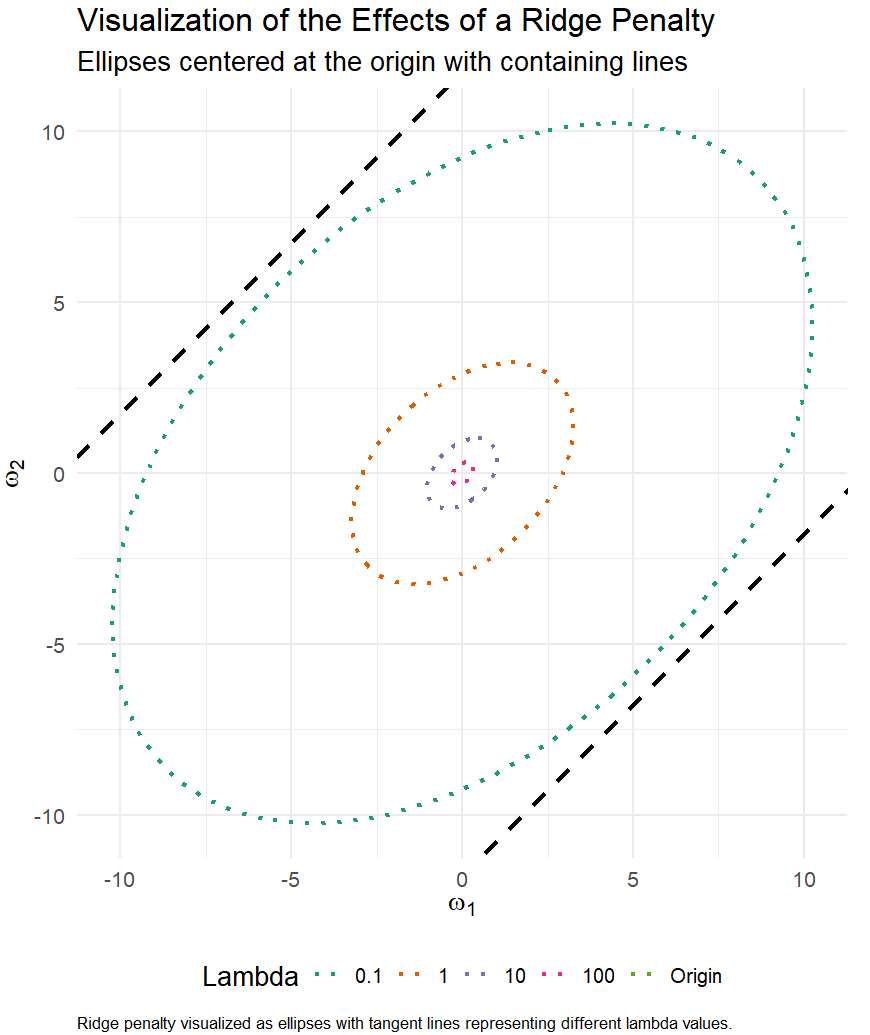
\includegraphics[width=0.9\textwidth]{visuals/ridge_effect_plot_bigger_dots.png}
    \caption{This plot illustrates the impact of ridge regularization in parameter space, where each ellipse represents a contour of equal penalized loss for different values of $\lambda$. As $\lambda$ increases, the ellipses, which are centered at the origin, become smaller, indicating stronger penalization and thus smaller coefficient values. The dashed lines represent the $ \lambda = 0 $ constraint. This visualization helps in understanding how ridge regression controls the complexity of the model by constraining the magnitude of the coefficients, effectively trading off a slight increase in bias for a significant reduction in variance \cite{Statlect2023Ridge}}
    \label{fig:tps}
\end{figure}
